\documentclass[10pt]{beamer}

\usetheme[progressbar=frametitle]{metropolis}
\usepackage{appendixnumberbeamer}

\usepackage{booktabs}
\usepackage[scale=2]{ccicons}
\usepackage{array}

\usepackage{pgfplots}
\usepgfplotslibrary{dateplot}

\usepackage{xspace}
\newcommand{\themename}{\textbf{\textsc{metropolis}}\xspace}
\graphicspath{{assets/}}

\title{TACO-Gold}
\subtitle{From Trump Retreat Risk to Gold Forecasting}
\date{}
\author{Horace et al.}
\institute{Project Presentation}

\begin{document}

\maketitle

\begin{frame}{Table of contents}
  \setbeamertemplate{section in toc}[sections numbered]
  \tableofcontents
\end{frame}

\section{Introduction}
\begin{frame}{Gold Price and Selected Trump Retreat Episodes}
  \begin{figure}
    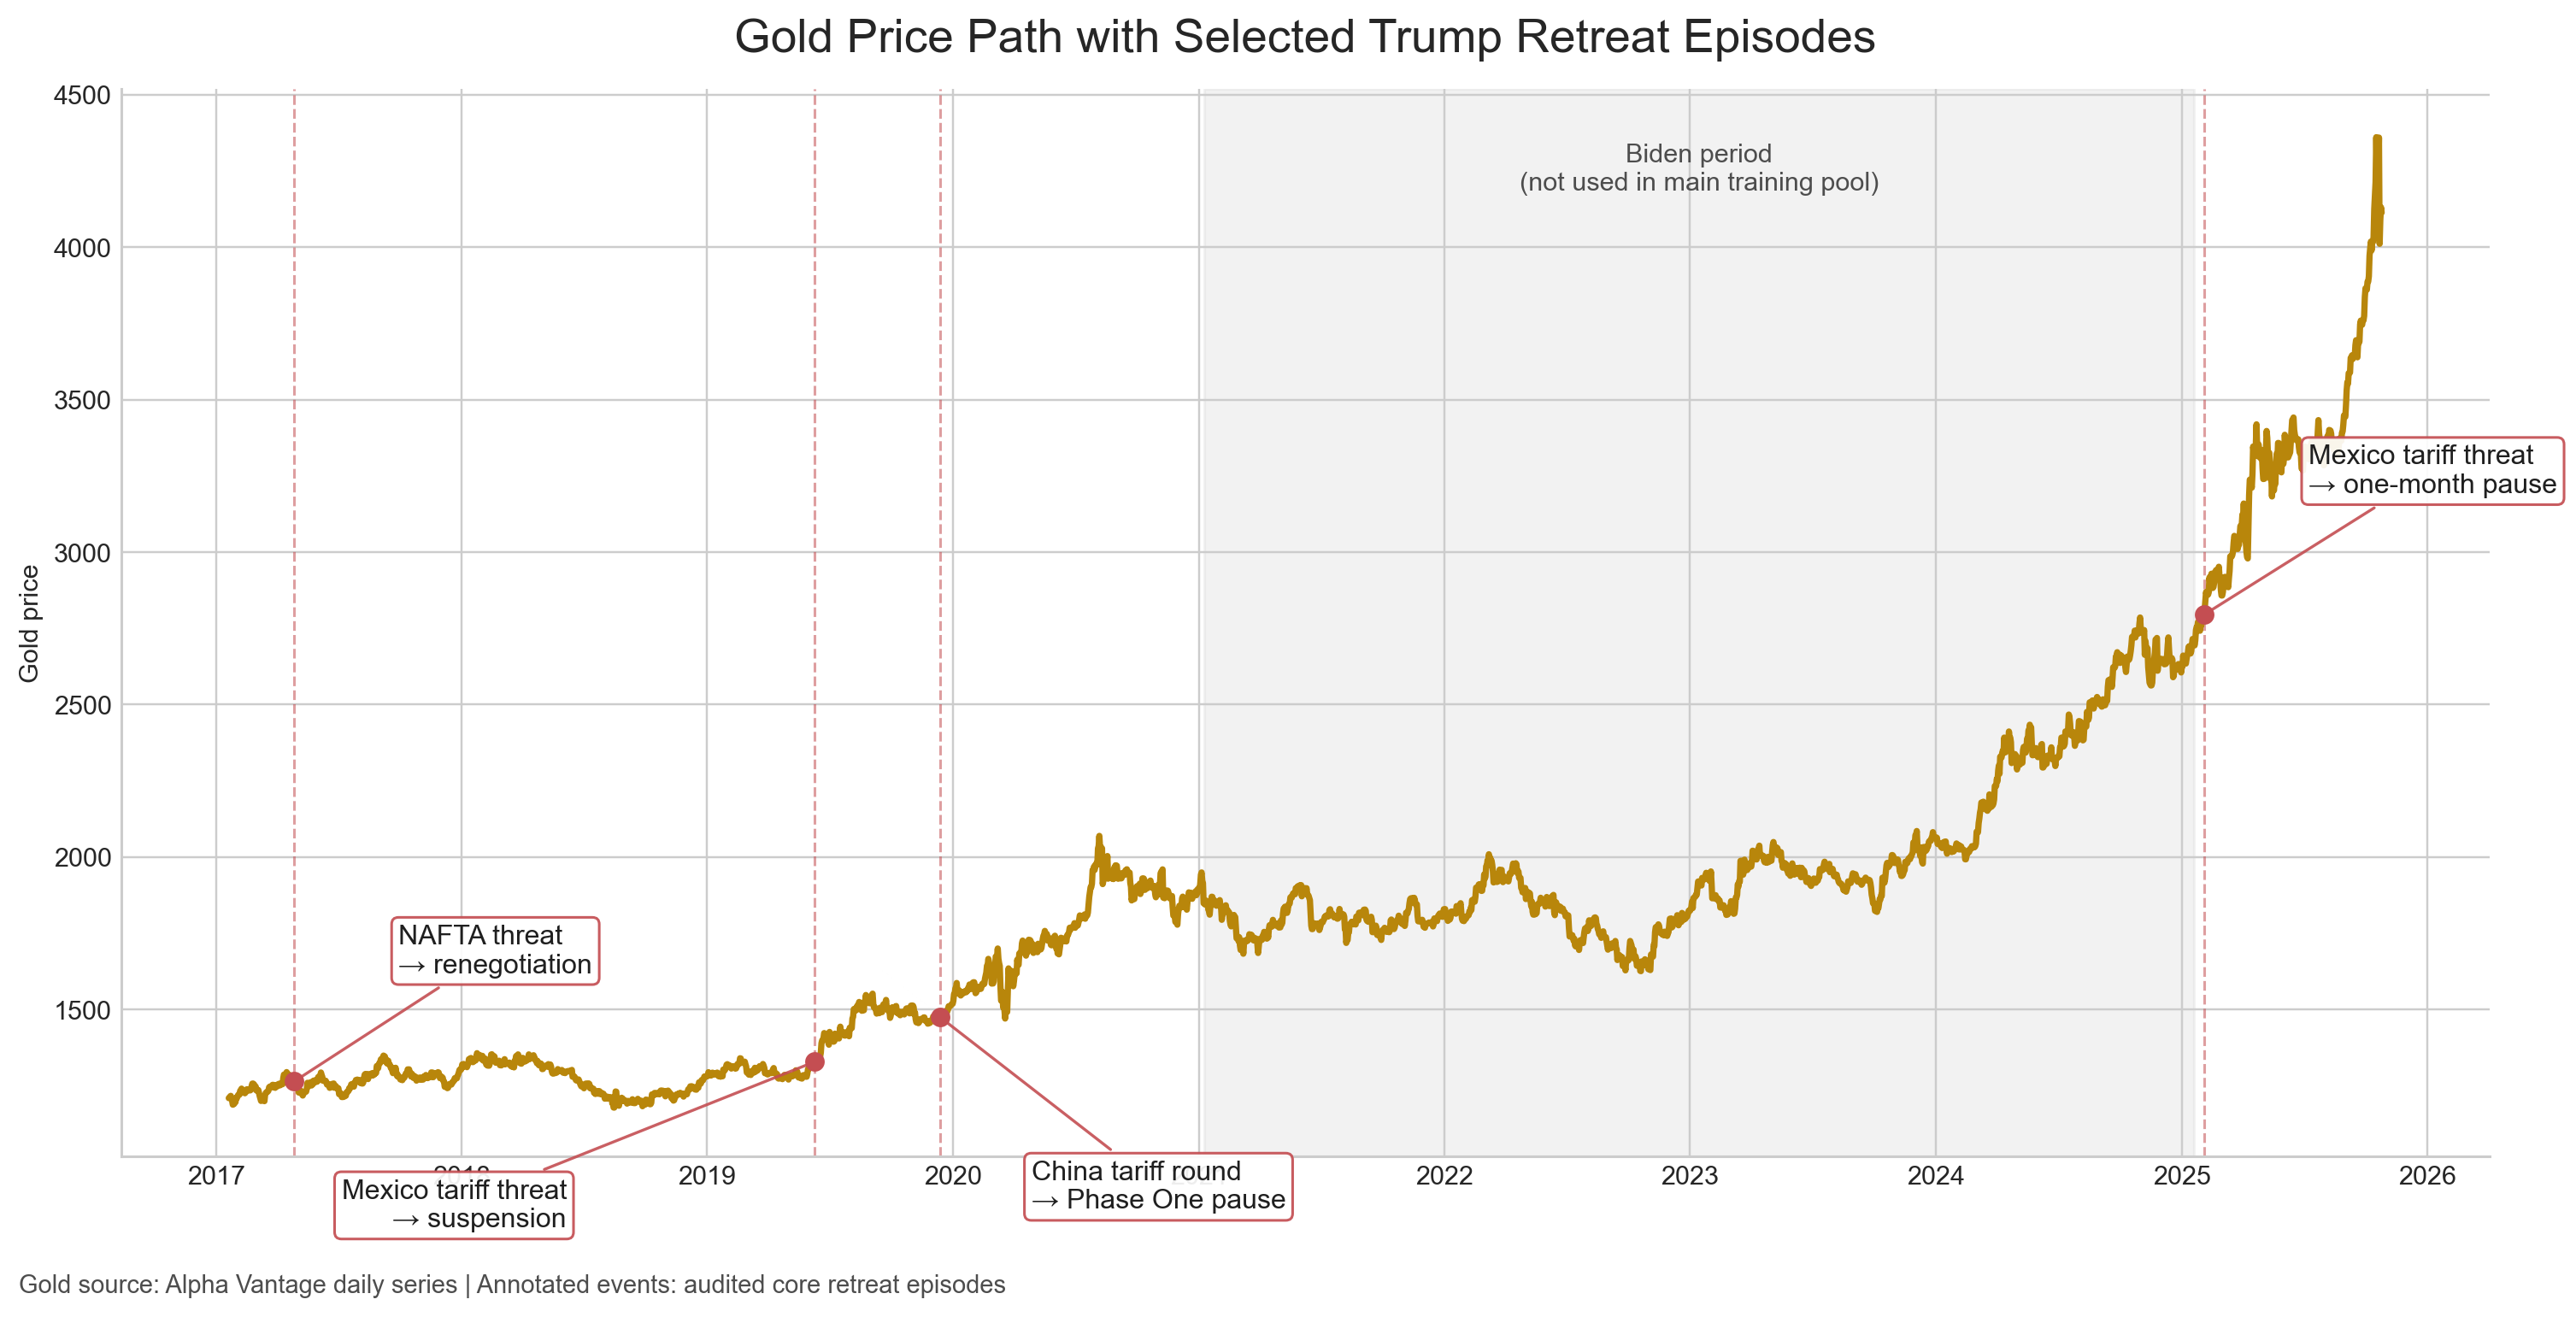
\includegraphics[width=\textwidth,height=0.78\textheight,keepaspectratio]{assets/gold_price_annotated_trump_episodes.png}
  \end{figure}

  \vspace{-0.4em}
  \small
  Trump's pressure-then-soften episodes often coincide with visible gold repricing. This motivates our core question: can we turn that pattern into a useful forecasting signal?
\end{frame}

\begin{frame}{Research Questions}
  \normalsize
  \small
  \textbf{TACO}: \emph{Trump Always Chickens Out}. It refers to Trump's tendency to back off after pressure or tariff threats.

  \vspace{0.7em}
  \normalsize
  {\bfseries\normalsize Question 1}\par
  \vspace{0.1em}
  \normalsize
  Can Trump's ``pressure-then-soften'' text pattern be transformed into a tradable signal?

  \vspace{0.8em}
  {\bfseries\normalsize Question 2}\par
  \vspace{0.1em}
  Can that signal improve gold-return forecasting beyond standard macro and market information?

  \vfill
  {\color{orange!90!black}\bfseries\normalsize Working Pipeline}\par
  \vspace{0.1em}
  \small
  Text pattern $\rightarrow$ event-level probability \texttt{P\_taco} $\rightarrow$ gold return forecasting
\end{frame}

\begin{frame}{What Exactly Are We Modeling?}
  \begin{block}{Not the broad popular claim}
    We are \alert{not} trying to model the vague statement that Trump ``often TACO'' in a general political sense.
  \end{block}

  \begin{block}{Operational definition in this project}
    \begin{itemize}
      \item Start from a pressure-like anchor text
      \item Observe Trump's own follow-up public texts within the next \textbf{48 hours}
      \item Detect whether a retreat signal appears: pause, delay, exemption, narrowing, or a shift toward negotiation
    \end{itemize}
  \end{block}

  \vspace{0.4em}
  Output: event-level probability \texttt{P\_taco}
\end{frame}


\section{Data and Labeling}
\begin{frame}{Data Sources}
  \small
  \begin{table}
    \centering
    \renewcommand{\arraystretch}{1.35}
    \begin{tabular}{>{\raggedright\arraybackslash}p{0.28\textwidth} >{\raggedright\arraybackslash}p{0.35\textwidth} >{\raggedright\arraybackslash}p{0.23\textwidth}}
      \toprule
      Data block & What we collect & Primary source \\
      \midrule
      Trump first-term text & Tweets, timestamps, raw text & Kaggle dataset \\
      Trump second-term text & Truth Social posts, timestamps, raw text & Public GitHub archive \\
      Market stress & SPX drawdown, VIX change, related controls & FRED \\
      Gold target series & Gold daily close and return series & Alpha Vantage \\
      Attention proxy & Tariff / war / inflation search attention & Google Trends \\
      \bottomrule
    \end{tabular}
  \end{table}

  \vspace{0.4em}
  \tiny
  Note: The second-term Truth Social archive comes from the public GitHub project \texttt{stiles/trump-truth-social-archive}.
\end{frame}

\begin{frame}{Sample Split and Labeling}
  \begin{columns}[T,onlytextwidth]
    \column{0.54\textwidth}
      \begin{block}{Training and Test Windows}
        \begin{itemize}
          \item First-term training window: \texttt{2017-01-20} to \texttt{2021-01-08}
          \item Second-term training window: \texttt{2025-01-20} to \texttt{2025-07-31}
          \item Test set / primary holdout: \texttt{2025-08-01} to \texttt{2025-10-25}
        \end{itemize}
      \end{block}

      \small
      Biden-period observations and the platform gap are excluded from the main training and test design.

    \column{0.42\textwidth}
      \begin{block}{Stage 1 Sample}
        \begin{itemize}
          \item Total events: \textbf{1,886}
          \item Positive events: \textbf{61}
          \item Positive rate: \textbf{3.23\%}
        \end{itemize}
      \end{block}

      \begin{block}{Labeling}
        \small
        Labels are assisted by \textbf{DeepSeek + prompt} to judge whether a retreat signal appears in the 48-hour follow-up texts.
      \end{block}
  \end{columns}
\end{frame}

\begin{frame}{Why Stage 1 Is a Rare-Event Problem}
  \begin{columns}[T,onlytextwidth]
    \column{0.48\textwidth}
      \centering
      {\bfseries\large Typical balanced\\classification\par}
      \vspace{0.55em}
      \begin{minipage}{0.92\linewidth}
        \begin{itemize}
          \item Positive and negative classes are closer in size
          \item Accuracy and ROC-style metrics are often informative
          \item The goal is usually overall classification correctness
        \end{itemize}
      \end{minipage}

    \column{0.48\textwidth}
      \centering
      {\color{orange!90!black}\bfseries\large Our Stage 1 task\par}
      \vspace{1.2em}
      \begin{minipage}{0.92\linewidth}
        \begin{itemize}
          \item Positive events are very rare (\(<5\%\))
          \item We care about ranking the few important positives near the top
          \item \textbf{PR-AUC} is more useful than plain accuracy here
        \end{itemize}
      \end{minipage}
  \end{columns}

  \vspace{0.5em}
  \small
  Intuition: PR-AUC focuses on whether the model's high-risk predictions are truly positive and whether rare positive cases are captured early.
\end{frame}

\begin{frame}{How We Handle the Rare-Event Setting}
  \begin{itemize}
    \item \textbf{Reweighting:} increase the importance of rare positives during training.
    \item \textbf{Selection metric:} compare models mainly with \textbf{PR-AUC}.
    \item \textbf{Calibration:} make the final \texttt{P\_taco} usable as a probability signal.
  \end{itemize}

  \begin{block}{Model-level handling}
    \begin{itemize}
      \item Linear models: class reweighting to improve sensitivity to rare positives
      \item Tree models: loss weighting based on the positive/negative class ratio
      \item Final comparison: probability quality rather than only hard-label accuracy
    \end{itemize}
  \end{block}

  \tiny
  References: King and Zeng (2001); Saito and Rehmsmeier (2015).
\end{frame}


\section{Method}
\begin{frame}{Validation Design and Leakage Control}
  \begin{itemize}
    \item \textbf{Nested CV}: model tuning and model comparison are separated.
    \item \textbf{OOF probabilities}: Stage 2 only consumes Stage 1 out-of-fold or true holdout probabilities.
    \item \textbf{Primary holdout}: \texttt{2025-08-01} to \texttt{2025-10-25} is reserved for final out-of-sample reporting.
    \item \textbf{Purged CV + embargo}: used to reduce neighboring-sample contamination and boundary leakage.
    \item \textbf{Lagged controls}: macro and market variables are lagged so only information available before the target day enters prediction.
  \end{itemize}

  \hspace{1.4em}
  \begin{minipage}{0.86\textwidth}
    \begin{alertblock}{Key rule}
      Stage 2 never uses in-sample Stage 1 probabilities.
    \end{alertblock}
  \end{minipage}
\end{frame}

\begin{frame}{Why a Two-Stage Design?}
  \begin{columns}[T,onlytextwidth]
    \column{0.47\textwidth}
      \centering
      {\bfseries\Large One-stage\par}
      \vspace{0.4em}
      Raw text sentiment aggregation\\[0.5em]
      $\Downarrow$\\[0.5em]
      Gold return prediction

    \column{0.47\textwidth}
      \centering
      {\color{orange!90!black}\bfseries\Large Two-stage\par}
      \vspace{0.4em}
      Text + pressure features\\[0.4em]
      $\Downarrow$\makebox[0pt][l]{\hspace{0.7em}\raisebox{0.25em}{\scriptsize Stage 1}}\\[0.45em]
      Event-level \texttt{P\_taco}\\[0.4em]
      $\Downarrow$\makebox[0pt][l]{\hspace{0.7em}\raisebox{0.25em}{\scriptsize Stage 2}}\\[0.45em]
      Gold return prediction
  \end{columns}

  \vspace{0.6em}
  \small
  Stage 1 acts as a \textbf{supervised signal compression} step: it turns noisy text into a task-aligned intermediate probability signal.
\end{frame}

\begin{frame}{What Goes into Stage 1?}
  \scriptsize
  \begin{table}
    \centering
    \begin{tabular}{p{0.24\textwidth} p{0.31\textwidth} p{0.33\textwidth}}
      \toprule
      Feature family & Examples & Role \\
      \midrule
      Text sentiment & FinBERT \texttt{pos / neu / neg} & Capture the semantic tone of the anchor text \\
      Candidate intensity & Keyword score, candidate priority, follow-up density & Describe whether the anchor looks like a strong pressure event \\
      Event metadata & Source, timing, term identifier & Preserve contextual event information \\
      Pressure features & SPX stress, VIX-related pressure signals & Capture market conditions around the event \\
      Attention proxy & Tariff / war / inflation attention & Optional public-attention signal \\
      \bottomrule
    \end{tabular}
  \end{table}

  \vspace{0.4em}
  \small
  FinBERT provides \textbf{positive / neutral / negative} probabilities for each anchor text. These are Stage 1 input features, not the final gold-forecast output.
\end{frame}

\begin{frame}{Stage 1 Result: Can We Learn a Usable \texttt{P\_taco}?}
  \footnotesize
  \begin{table}
    \centering
    \renewcommand{\arraystretch}{1.15}
    \begin{tabular}{>{\raggedright\arraybackslash}p{0.07\textwidth}
                    >{\raggedright\arraybackslash}p{0.22\textwidth}
                    >{\raggedright\arraybackslash}p{0.14\textwidth}
                    r r r}
      \toprule
      Rank & Model & Prob. & PR-AUC & Brier & ECE \\
      \midrule
      \textbf{1} & \textbf{linear\_svm} & \textbf{sigmoid} & \textbf{0.0837} & \textbf{0.0442} & \textbf{0.0218} \\
      2 & linear\_svm & isotonic & 0.0679 & 0.0448 & 0.0302 \\
      3 & xgboost\_classifier & sigmoid & 0.0464 & 0.0448 & 0.0250 \\
      4 & xgboost\_classifier & isotonic & 0.0649 & 0.0455 & 0.0278 \\
      5 & logistic\_regression & isotonic & 0.0735 & 0.0456 & 0.0309 \\
      6 & logistic\_regression & sigmoid & 0.0669 & 0.0461 & 0.0280 \\
      7 & xgboost\_classifier & raw & 0.0621 & 0.0531 & 0.0534 \\
      8 & logistic\_regression & raw & 0.0856 & 0.2601 & 0.4520 \\
      \bottomrule
    \end{tabular}
  \end{table}

  \vspace{0.4em}
  \small
  Best probability variant under the outer-CV selection rule: \textbf{linear\_svm + sigmoid}

  \tiny
  Note: although \texttt{logistic\_regression raw} has a high PR-AUC, its probability quality is much worse in Brier and ECE, so it is not selected.
\end{frame}

\begin{frame}{What Goes into Stage 2?}
  \footnotesize
  \begin{table}
    \centering
    \renewcommand{\arraystretch}{1.18}
    \begin{tabular}{>{\raggedright\arraybackslash}p{0.25\textwidth} >{\raggedright\arraybackslash}p{0.56\textwidth}}
      \toprule
      Feature family & Representative inputs \\
      \midrule
      Daily \texttt{P\_taco} aggregates & \texttt{p\_taco\_any}, \texttt{p\_taco\_top1}, \texttt{p\_taco\_tail\_010}, \texttt{p\_taco\_any\_decay\_2d} \\
      Lagged macro / market controls & DXY return, real yield change, VIX, SPX stress \\
      Cross-asset structure & Gold-SPX rolling correlation \\
      \bottomrule
    \end{tabular}
  \end{table}

  \vspace{0.6em}
  \begin{block}{Target definition}
    \[
    \mathrm{Gold\_Return}_e=
    \log\left(
    \frac{\mathrm{GoldClose}_{\tau(e)}}{\mathrm{GoldClose}_{a(e)}}
    \right)
    \]

    \vspace{0.2em}
    \footnotesize
    \begin{itemize}
      \item $\tau(e)$: first valid trading day after the event
      \item $a(e)$: nearest valid trading day before the event
    \end{itemize}
  \end{block}
\end{frame}

\begin{frame}{Stage 2 Final Model Selection}
  \footnotesize
  \begin{table}
    \centering
    \renewcommand{\arraystretch}{1.15}
    \begin{tabular}{>{\raggedright\arraybackslash}p{0.10\textwidth}
                    >{\raggedright\arraybackslash}p{0.22\textwidth}
                    r r}
      \toprule
      Rank & Model & RMSE & MAE \\
      \midrule
      \textbf{1} & \textbf{RF} & \textbf{0.0098} & \textbf{0.0072} \\
      2 & Ridge & 0.0099 & 0.0072 \\
      3 & XGB & 0.0100 & 0.0074 \\
      \bottomrule
    \end{tabular}
  \end{table}

  \vspace{0.4em}
  \small
  Final selection is based on \textbf{outer-CV RMSE and MAE}; the holdout is used only for final out-of-sample reporting.

  \vspace{0.25em}
  \small
  Selected model: \texttt{svm\_sigmoid + RF + two\_stage\_v2\_core}

  \tiny
  Holdout RMSE comparison: RF = 0.0153, Ridge = 0.0156, XGB = 0.0153.
\end{frame}

\begin{frame}{Interpretation: What Does the Final Model Use?}
  \begin{figure}
    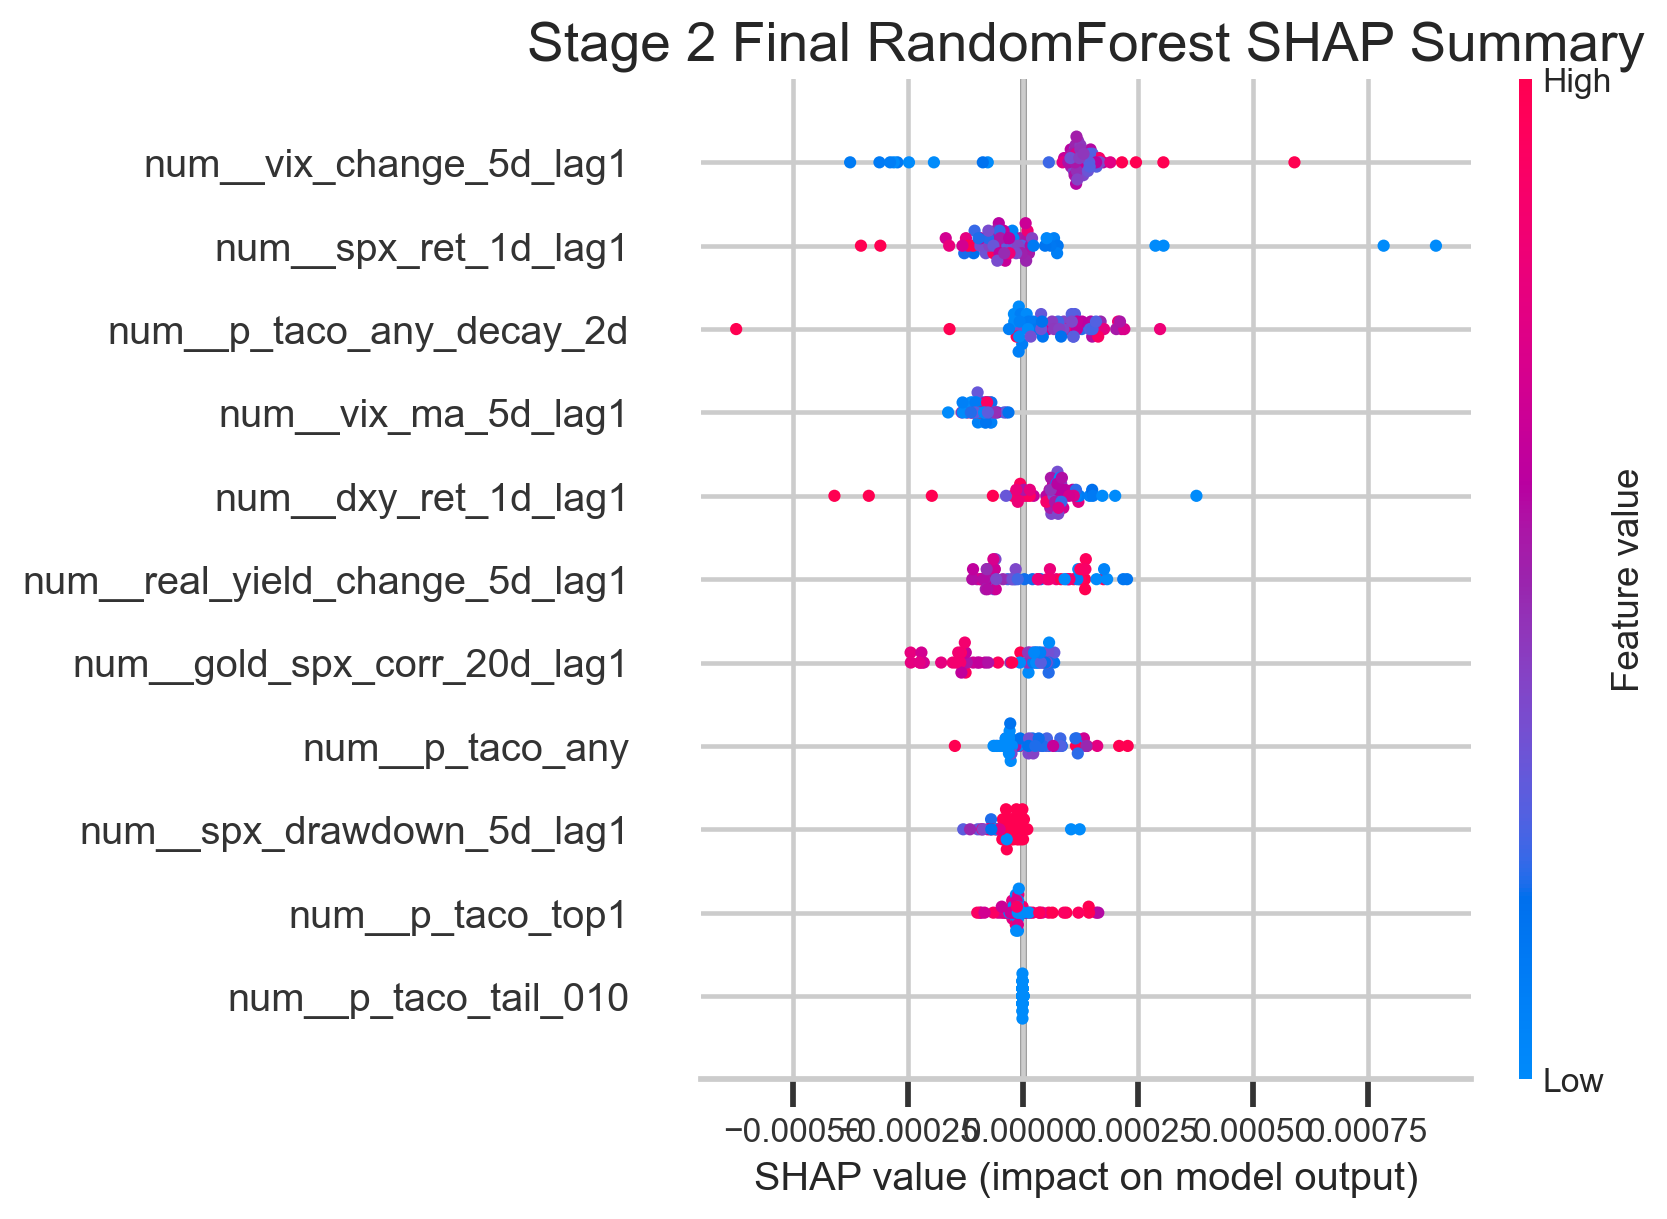
\includegraphics[width=0.86\textwidth,height=0.62\textheight,keepaspectratio]{stage2_rf_shap_summary.png}
  \end{figure}

  \small
  \texttt{P\_taco}-related features enter the important-feature layer together with lagged macro-financial controls, suggesting that the signal is not merely duplicating standard market information.
\end{frame}


\section{Results}
\begin{frame}{Main Result I: Does the Signal Add Value Beyond Standard Baselines?}
  \footnotesize
  \begin{table}
    \centering
    \renewcommand{\arraystretch}{1.15}
    \begin{tabular}{>{\raggedright\arraybackslash}p{0.28\textwidth} r r r r}
      \toprule
      Benchmark & RMSE & MAE & $R^2$ & Sign Acc. \\
      \midrule
      Random Walk & 0.015593 & 0.009891 & -0.061624 & 0.000000 \\
      Macro-only Linear & 0.015593 & 0.009773 & -0.061553 & 0.590164 \\
      Macro-only Tree & 0.015432 & 0.009682 & -0.039723 & \textbf{0.688525} \\
      \textbf{Two-stage Main Model} & \textbf{0.015349} & \textbf{0.009605} & \textbf{-0.028609} & 0.672131 \\
      \bottomrule
    \end{tabular}
  \end{table}

  \vspace{0.4em}
  \small
  This slide answers the first research question. The two-stage main model improves on random walk and linear macro baselines, and delivers the best overall RMSE among the benchmark set.

  \tiny
  Holdout RMSE: two-stage = 0.015349 vs macro-only comparator = 0.015409.
\end{frame}

\begin{frame}{Main Result II: Is Two-Stage Better Than Direct Text-to-Return Modeling?}
  \begin{figure}
    \centering
    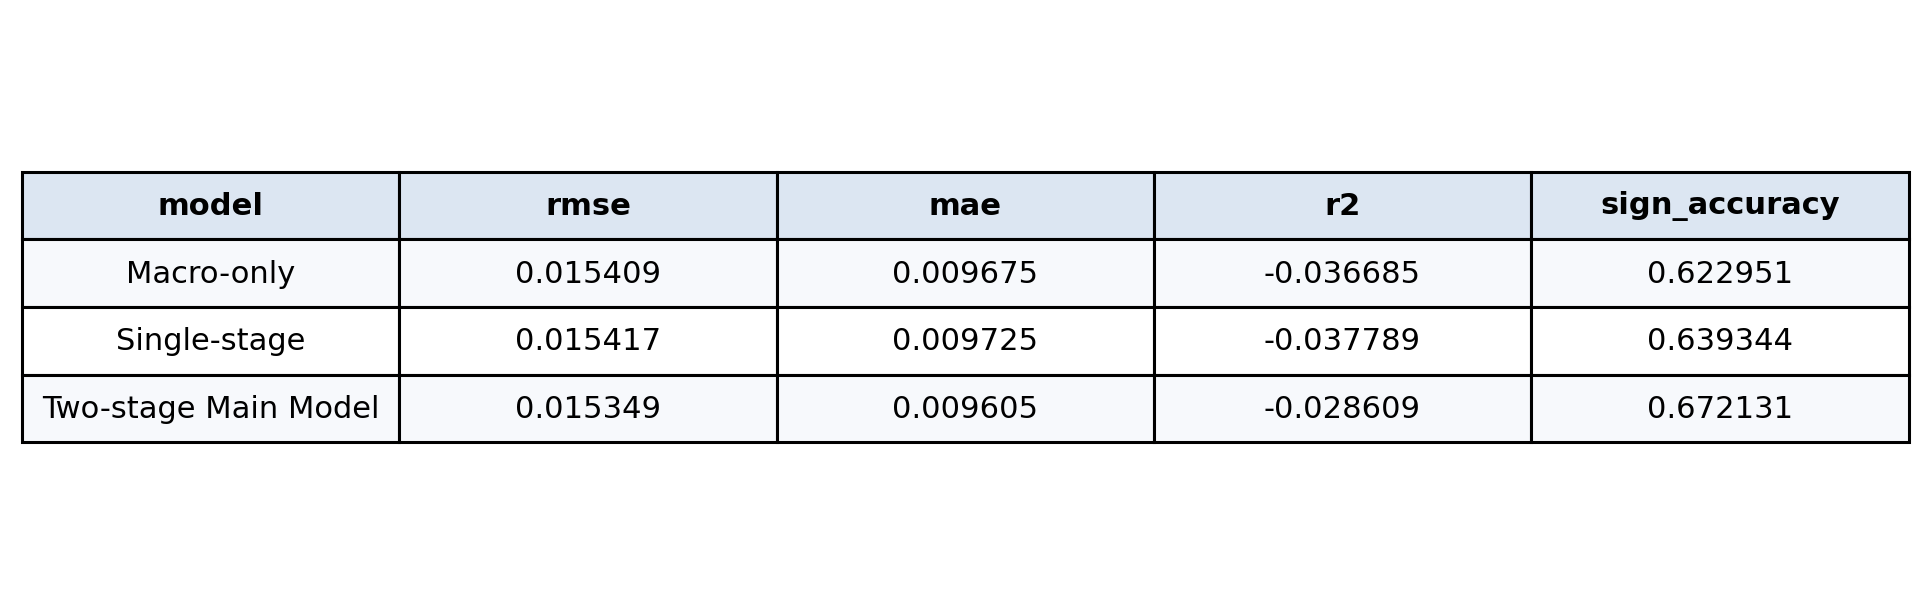
\includegraphics[width=0.72\textwidth]{two_stage_vs_single_stage_table.png}
  \end{figure}

  \vspace{0.35em}
  \small
  This slide answers the second research question. In the final comparison, the ordering is:

  \vspace{0.25em}
  \centering
  \textbf{direct text < macro-only < two-stage}
\end{frame}

\begin{frame}{Why Is the Out-of-Sample \texorpdfstring{$R^2$}{R2} Negative?}
  \begin{block}{Out-of-sample \texorpdfstring{$R^2$}{R2} formula}
    \[
    R^2_{\mathrm{oos}}
    =
    1-
    \frac{\sum_{t \in \mathrm{test}} (y_t-\hat{y}_t)^2}
         {\sum_{t \in \mathrm{test}} (y_t-\bar{y}_{\mathrm{test}})^2}
    \]
  \end{block}

  \begin{alertblock}{When is it negative?}
    \[
    R^2_{\mathrm{oos}} < 0
    \quad \Longleftrightarrow \quad
    \sum (y_t-\hat{y}_t)^2
    >
    \sum (y_t-\bar{y}_{\mathrm{test}})^2
    \]
    In words: the model's test-set squared error is larger than the squared error from simply predicting the holdout mean.
  \end{alertblock}

  \begin{itemize}
    \item Gold daily returns are noisy, so negative holdout $R^2$ is not unusual in short forecasting windows.
    \item A negative $R^2$ does \alert{not} mean the model is useless; it means it fails to beat the holdout-mean baseline under squared-error loss.
    \item In this project, \textbf{RMSE}, \textbf{MAE}, and directional accuracy are more informative summary metrics than $R^2$ alone.
  \end{itemize}

  \tiny
  Final two-stage holdout $R^2 = -0.0286$.
\end{frame}


\section{Conclusion}
\begin{frame}{Conclusion}
  \begin{block}{Answer to our research questions}
    \begin{enumerate}
      \item We can operationalize Trump's short-horizon pressure-then-soften pattern into an event-level probability signal, \texttt{P\_taco}.
      \item That signal provides incremental information beyond standard macro and market controls.
      \item A two-stage structure works better than direct text aggregation for this forecasting task.
    \end{enumerate}
  \end{block}

  \small
  These conclusions should be understood under the current definition, sample boundary, and validation protocol.
\end{frame}


\appendix
\begin{frame}{Appendix: Validation Protocol Backup}
  \begin{itemize}
    \item Outer CV determines the final model comparison.
    \item Inner CV handles model-specific tuning.
    \item Stage 1 probabilities passed to Stage 2 are always OOF or true holdout predictions.
    \item Purged CV and embargo reduce nearby-sample contamination.
    \item Lagged macro / market controls preserve time-availability discipline.
  \end{itemize}
\end{frame}

\begin{frame}{Appendix: Labeling Logic Backup}
  \begin{itemize}
    \item Start from candidate pressure-like events.
    \item For each anchor event, inspect Trump's own follow-up texts within the next 48 hours.
    \item Use DeepSeek-assisted prompting to judge whether a retreat signal appears.
    \item The final Stage 1 target is therefore an operational \textit{text-observed retreat} label.
  \end{itemize}
\end{frame}


\end{document}
